\chapter{Response Rigidity, Symmetry, and Curvature}\label{ch:rigidity}

\section{Anchored response geometry}
Let $p$ vary in an interval containing a parity symmetric point $p_0$. Let
\begin{equation}
 Z(p)=x(p)+iy(p)\ne0
 \label{eq:rig_z}
\end{equation}
be the measured complex shear response under a fixed response prescription. Assume the anchor is real and positive,
\begin{equation}
 Z(p_0)=x_0>0.
 \label{eq:rig_anchor}
\end{equation}
The circle whose diameter joins $0$ to $x_0$ on the real axis has equation
\begin{equation}
 \left(x-\frac{x_0}{2}\right)^2+y^2
 =\left(\frac{x_0}{2}\right)^2.
 \label{eq:rig_circle_center}
\end{equation}
Equivalently,
\begin{equation}
 x^2+y^2=x_0x.
 \label{eq:rig_circle}
\end{equation}
Define the signed algebraic defect
\begin{equation}
 \Delta(p)=|Z(p)|^2-x_0\RePart Z(p).
 \label{eq:rig_delta}
\end{equation}
Circle membership is exactly the zero set $\Delta=0$.

\section{Closure free classification theorem}
Since $Z\ne0$,
\begin{equation}
 \RePart\!\left(\frac1Z\right)
 =\frac{\RePart Z}{|Z|^2}.
 \label{eq:rig_inverse_real}
\end{equation}
Divide \cref{eq:rig_delta} by $|Z|^2$ to obtain
\begin{equation}
 \frac{\Delta}{|Z|^2}
 =1-x_0\RePart\!\left(\frac1Z\right).
 \label{eq:rig_master_identity}
\end{equation}
At the anchor, $1/Z(p_0)=1/x_0$. Therefore:

\paragraph{Response rigidity theorem.}
For every nonzero complex response satisfying \cref{eq:rig_anchor},
\begin{equation}
 \Delta(p)=0
 \quad\Longleftrightarrow\quad
 \RePart\!\left(\frac1{Z(p)}\right)
 =\RePart\!\left(\frac1{Z(p_0)}\right).
 \label{eq:rig_theorem}
\end{equation}

The proof is the identity \cref{eq:rig_master_identity}. No simulation, kinetic closure, collision model, or fixed response prefactor is required. The theorem classifies membership in one specified anchored circle. It does not say that every curve of constant curvature is this circle, nor that every generalized circle must pass through the anchor and origin.

\begin{figure}[htbp]
\centering
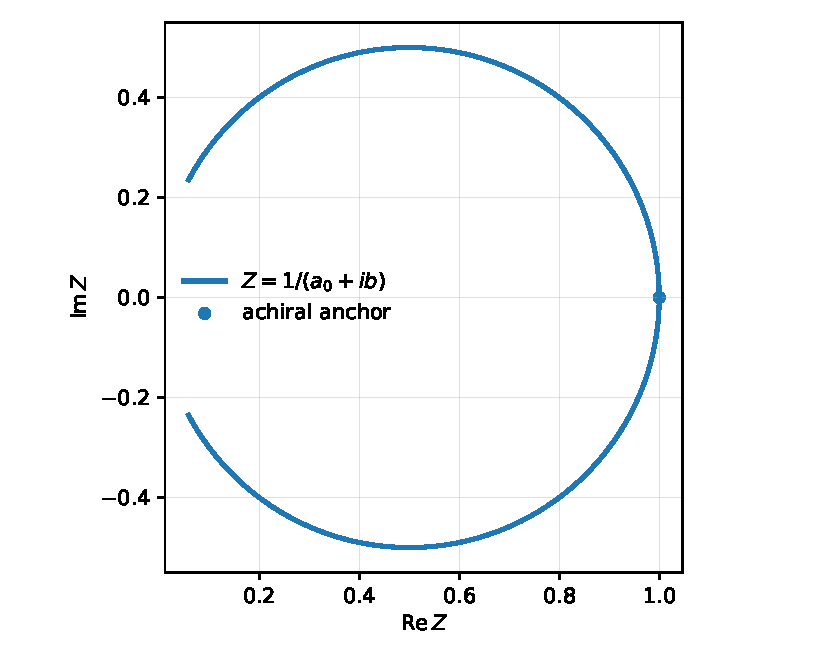
\includegraphics[width=.72\textwidth]{inverse_response_geometry.pdf}
\caption{Complex inversion of the vertical inverse response locus $\RePart(1/Z)=a_0$ produces the anchored circle. The plotted curve uses $a_0=1$ and is generated analytically from $Z=1/(a_0+i b)$.}
\label{fig:inverse_geometry}
\end{figure}

\section{Kernel coordinates and the defect formula}
Write the measured inverse response as
\begin{equation}
 Q(p)=\frac1{Z(p)}=a(p)+ib(p),
 \label{eq:q_ab}
\end{equation}
and define
\begin{equation}
 a_0=a(p_0)=\frac1{x_0}.
 \label{eq:a0}
\end{equation}
Then
\begin{equation}
 Z=\frac{a-ib}{a^2+b^2},
 \qquad
 |Z|^2=\frac{1}{a^2+b^2}.
 \label{eq:z_ab}
\end{equation}
Substitution into \cref{eq:rig_delta} gives
\begin{equation}
 \boxed{
 \Delta(p)=\frac{a_0-a(p)}{a_0\left[a(p)^2+b(p)^2\right]}}
 \label{eq:defect_ab}
\end{equation}
for the normalized measured response.

Several consequences follow immediately. Arbitrary changes of the reactive coordinate $b(p)$ preserve the circle if $a(p)=a_0$. Any drift of $a$ away from $a_0$ produces a nonzero defect. Within this two coordinate description there is no third class for the membership predicate: a point is either on the anchored circle because the inverse real part equals $a_0$, or it is off that circle because the inverse real part differs.

If a model is instead parameterized as
\begin{equation}
 Z(p)=\frac{A(p)}{\alpha(p)+i\beta(p)},
 \label{eq:prefactor_model}
\end{equation}
then
\begin{equation}
 \RePart\!\left(\frac1Z\right)=\frac{\alpha(p)}{A(p)}.
 \label{eq:prefactor_ratio}
\end{equation}
It is therefore not correct in general to identify rigidity with constant $\alpha$ alone. The closure free theorem is written in terms of the actual measured $1/Z$ precisely to absorb any response residue or normalization into the observable quantity.

\section{Sixfold symmetry and the shear commutant}
The traceless symmetric shear components in two dimensions form a real two component representation. A physical rotation through angle $\theta$ acts on this doublet through angle $2\theta$. For a nontrivial element of $C_6$, one may use the $120$ degree matrix
\begin{equation}
 R=\begin{pmatrix}
 -\tfrac12&-\tfrac{\sqrt3}{2}\\
 \tfrac{\sqrt3}{2}&-\tfrac12
 \end{pmatrix}.
 \label{eq:c6_rotation}
\end{equation}
Let
\begin{equation}
 M=\begin{pmatrix}m_{11}&m_{12}\\m_{21}&m_{22}\end{pmatrix}
 \label{eq:generic_m}
\end{equation}
be a real linear operator that commutes with $R$. Solving $MR=RM$ gives
\begin{equation}
 m_{11}=m_{22},
 \qquad
 m_{12}=-m_{21}.
 \label{eq:commutant_constraints}
\end{equation}
Thus
\begin{equation}
 M=aI+bJ,
 \qquad
 J=\begin{pmatrix}0&-1\\1&0\end{pmatrix}.
 \label{eq:commutant_form}
\end{equation}
The independent symbolic audit solves this commutator equation directly and verifies that the commutant is two dimensional.

Reflection conjugates $J$ to $-J$. If chirality displacement $d=p-p_0$ changes sign under reflection, covariance implies the parity structure
\begin{equation}
 a(d)=a(-d),
 \qquad
 b(d)=-b(-d).
 \label{eq:parity_ab}
\end{equation}
This is not enough to make $a$ constant. Terms such as $a_2d^2$, $a_4d^4$, and higher even powers are symmetry allowed. Sixfold symmetry gives the complex scalar form, while rigidity is an additional condition.

\section{Curvature of the response map}
The response map is a plane curve $r(d)=(x(d),y(d))$. Its signed curvature for a regular parameterization is
\begin{equation}
 \kappa(d)=
 \frac{x'(d)y''(d)-y'(d)x''(d)}
 {\left[x'(d)^2+y'(d)^2\right]^{3/2}}.
 \label{eq:curvature_general}
\end{equation}
Assume parity near $d=0$ and expand
\begin{equation}
 a(d)=a_0+\frac{a_2}{2}d^2+O(d^4),
 \qquad
 b(d)=b_1d+O(d^3),
 \label{eq:local_expansion}
\end{equation}
with $b_1>0$ setting the orientation. Substituting $Z=1/(a+ib)$ into \cref{eq:curvature_general} gives
\begin{equation}
 \boxed{
 \kappa(0)=-2a_0-\frac{a_0^2a_2}{b_1^2}}
 \label{eq:curvature_achiral}
\end{equation}
for the chosen orientation convention. In the rigid class $a_2=0$ and the anchored circle has radius $1/(2a_0)$, so its signed curvature is $-2a_0$.

Equation \cref{eq:curvature_achiral} makes the role of quadratic dissipative drift concrete. It also explains why curvature is useful as a local diagnostic. If $a_2\ne0$, the achiral curvature differs from the rigid circle value.

\section{Why local curvature is not a global classifier}
Curvature at one point cannot decide global circle membership. Consider
\begin{equation}
 a(d)=a_0+\epsilon d^4,
 \qquad
 b(d)=cd.
 \label{eq:quartic_drift}
\end{equation}
Then $a''(0)=0$, so \cref{eq:curvature_achiral} gives the same achiral curvature as the rigid circle. Nevertheless \cref{eq:defect_ab} becomes
\begin{equation}
 \Delta(d)=
 -\frac{\epsilon d^4}
 {a_0\left[(a_0+\epsilon d^4)^2+c^2d^2\right]},
 \label{eq:quartic_defect}
\end{equation}
which is nonzero for $d\ne0$ if $\epsilon\ne0$. The curve departs from the anchored circle while agreeing with its local curvature at the anchor.

This counterexample refines the role of the second fundamental form. Curvature is a meaningful local geometric observable and can detect leading dissipative drift, but the exact global classifier is \cref{eq:rig_theorem}. A theorem stated only as ``fixed curvature if and only if rigidity'' would be false without stronger hypotheses on the family of curves.

\section{Renormalization flow criterion}
The classification can be stated at every scale. Let $Z_\ell(p)$ be an effective response at scale $\ell$ and define
\begin{equation}
 a_\ell(p)=\RePart\!\left[\frac1{Z_\ell(p)}\right].
 \label{eq:scale_a}
\end{equation}
The circle preserving manifold is
\begin{equation}
 G_\ell(p)=a_\ell(p)-a_\ell(p_0)=0.
 \label{eq:rigid_manifold}
\end{equation}
If $\beta_a(p,\ell)=\partial_\ell a_\ell(p)$, local invariance of this manifold under the flow requires and, for a regular deterministic flow, is sufficient in the tangent sense that
\begin{equation}
 \beta_a(p,\ell)-\beta_a(p_0,\ell)=0
 \quad\text{whenever}\quad G_\ell(p)=0.
 \label{eq:rg_tangent}
\end{equation}
This equation describes exactly what an additional protection mechanism would need to enforce. $C_6$ symmetry by itself does not supply \cref{eq:rg_tangent}.

\section{Ward identity boundary}
The defect identity \cref{eq:rig_master_identity} is a consequence of algebra and complex inversion. It is therefore valid whether or not the microscopic model has a conservation law capable of protecting the rigid manifold. A genuine Ward identity interpretation would require a derivation in which a symmetry generator or conservation law implies \cref{eq:rg_tangent} or its exact microscopic equivalent. Established viscosity Ward identities provide examples of that logic in other settings \cite{Bradlyn2012}.

Until such a derivation is supplied for the correlated chiral FHP model, the correct language is response rigidity, not Ward protection. This distinction is part of the theorem rather than a disclaimer added afterward: symmetry fixes the allowed form of the kernel, while a separate condition fixes whether its dissipative coordinate is flat.

\section{Chapter conclusion}
The response circle problem has an exact closure free answer. The anchored circle survives precisely when the real part of the measured inverse response is constant relative to the achiral anchor. Sixfold symmetry explains why an isolated shear sector has two scalar coordinates, but it permits dissipative drift. Curvature detects some local departures but cannot replace the global inverse response criterion. The next chapter shows that the nonrigid class is physically admissible by constructing a stationary positive dissipation Green Kubo counterexample.
